\documentclass[11pt,letterpaper]{article}

% ---------- Paquetes ----------
\usepackage[utf8]{inputenc}
\usepackage[T1]{fontenc}
\usepackage[spanish,es-tabla]{babel}
\usepackage[margin=2.5cm]{geometry}
\usepackage{graphicx}
\usepackage{booktabs}
\usepackage{amsmath}
\usepackage{amssymb}
\usepackage{listings}
\usepackage{xcolor}
\usepackage{caption}
\usepackage{hyperref}
\usepackage{enumitem}
\usepackage{float}

\hypersetup{
    colorlinks=true,
    linkcolor=blue!50!black,
    citecolor=blue!50!black,
    urlcolor=blue!50!black,
    pdftitle={Capa de datos distribuida y pipeline analitico paralelo - Equipo ACC},
    pdfauthor={Carlos Carpio, Cristhian Pacheco, Robinson Cando, Jeremy Alvarez}
}

\definecolor{codebg}{RGB}{245,245,245}
\definecolor{codecomment}{RGB}{100,100,100}
\definecolor{codekeyword}{RGB}{0,0,180}
\definecolor{codestring}{RGB}{160,30,30}

\lstdefinestyle{codigo}{
    backgroundcolor=\color{codebg},
    commentstyle=\color{codecomment}\itshape,
    keywordstyle=\color{codekeyword}\bfseries,
    stringstyle=\color{codestring},
    basicstyle=\footnotesize\ttfamily,
    breakatwhitespace=false,
    breaklines=true,
    captionpos=b,
    keepspaces=true,
    numbers=left,
    numbersep=5pt,
    numberstyle=\tiny\color{codecomment},
    showspaces=false,
    showstringspaces=false,
    showtabs=false,
    tabsize=2,
    frame=single,
    rulecolor=\color{black!20}
}
\lstset{style=codigo}

\newcommand{\seccionpagref}[1]{} % placeholder, no-op

\title{\textbf{Capa de datos distribuida y pipeline anal\'itico paralelo}\\
\large Sistema de Gesti\'on de Solicitudes de Soporte T\'ecnico de Internet\\
\large Entrega 3 --- Aplicaciones Distribuidas (ISR-701)}

\author{
Carlos Jos\'e Carpio Mendoza \and
Cristhian Daniel Pacheco C\'ardenas \and
Robinson Rodrigo Cando Moreno \and
Jeremy \'Alvarez\\[1em]
\normalsize Equipo ACC\\
\normalsize Facultad de Ciencias de la Computaci\'on\\
\normalsize Universidad T\'ecnica Estatal de Quevedo
}

\date{Julio 2026}

\begin{document}

\maketitle

\begin{abstract}
\noindent
\textbf{Objetivo.} Consolidar la capa de datos distribuida y el pipeline analítico paralelo del
Sistema de Soporte Técnico ISP (equipo ACC), evaluando su rendimiento y tolerancia a fallos. \textbf{Método.} Se fragmentó \texttt{tickets} por rango de \texttt{fecha\_apertura} sobre un
clúster de tres nodos de CockroachDB, verificando completitud, reconstrucción y
disyunción~\cite{ozsu2011principles}; se instrumentó con métricas Prometheus validadas con
\texttt{promtool} y pruebas Testcontainers contra \texttt{SERIALIZABLE} real; y se rediseñó un
pipeline de Spark sobre 600{,}000 incidencias con cinco transformaciones, contrastado mediante
protocolo experimental (Jain~\cite{jain1991art}, Wohlin et al.~\cite{wohlin2012experimentation})
frente a un baseline en pandas.
\textbf{Resultados.} El clúster aplica correctamente aislamiento serializable ante escrituras
concurrentes conflictivas (\texttt{SQLSTATE 40001}), las tres métricas pasan el \emph{linter} de
Prometheus sin advertencias, y el pipeline detecta 380{,}753 incidencias reincidentes (68.3\%)
sobre 557{,}701 filas filtradas. El protocolo estadístico completo (50 corridas) muestra que,
para este volumen de datos, el baseline secuencial en pandas fue significativamente más rápido que
Spark incluso con ocho núcleos ($p \approx 5\times10^{-10}$), aunque Spark sí exhibe un
\emph{speedup} interno real al escalar de uno a ocho núcleos ($p$ de Amdahl $\approx 0.53$). El
clúster tolera la caída de un nodo sin pérdida de datos ni de disponibilidad de escritura (0
errores en 691 filas, pico de latencia P95 de 1.59\,s durante la reelección de líder), y pierde
disponibilidad de escritura durante 62\,s al caer dos de tres nodos, recuperándose de inmediato al
reincorporar un nodo. \textbf{Conclusión.} La fragmentación y la
instrumentación aplicadas son correctas y verificables; el protocolo revela además que el
paralelismo distribuido no es gratuito y solo se justifica a partir de cierta escala de datos.
\end{abstract}

\begin{center}\textbf{Abstract}\end{center}
\begin{abstract}
\noindent
\textbf{Objective.} To consolidate the distributed data layer and the parallel analytics pipeline
of the ISP Technical Support Ticket Management System (team ACC), evaluating their performance
and fault tolerance. \textbf{Method.}
The \texttt{tickets} table was fragmented by range on \texttt{fecha\_apertura} over a three-node
CockroachDB cluster, verifying completeness, reconstruction and
disjointness~\cite{ozsu2011principles}; the service was instrumented with Prometheus metrics
validated with \texttt{promtool} and Testcontainers tests against real \texttt{SERIALIZABLE}
isolation; and a Spark pipeline was redesigned over 600,000 incidents with five transformations,
contrasted via an experimental protocol against a pandas baseline. \textbf{Results.} The cluster correctly enforces
serializable isolation under conflicting concurrent writes (\texttt{SQLSTATE 40001}), all three
required metrics pass the Prometheus linter without warnings, and the pipeline detects 380,753
recurring incidents (68.3\%) out of 557,701 filtered rows. The full statistical protocol (50
trials) shows that, at this data volume, the sequential pandas baseline was significantly faster
than Spark even at eight cores ($p \approx 5\times10^{-10}$), although Spark does show a real
internal speedup when scaling from one to eight cores (Amdahl $p \approx 0.53$). The cluster
tolerates a single-node failure without data loss or write-availability loss (0 errors across 691
rows, peak P95 latency of 1.59\,s during leader re-election), and loses write availability for
62\,s when two of three nodes go down, recovering immediately once a node rejoins. \textbf{Conclusion.} The fragmentation and instrumentation
applied are correct and empirically verifiable; the protocol further reveals that distributed
parallelism is not free and only pays off past a certain data scale.
\end{abstract}


\tableofcontents
\newpage

\section{Introducción}
\label{sec:introduccion}

\subsection{Continuidad del proyecto}

El Sistema de Gestión de Solicitudes de Soporte Técnico de Internet es el proyecto final de
carrera del equipo ACC para la asignatura de Aplicaciones Distribuidas. En la Entrega 1 se
definió el dominio del problema —un proveedor de servicios de Internet (ISP) que necesita
registrar, clasificar, asignar y dar seguimiento a solicitudes de soporte técnico de sus
clientes— y se construyó un primer prototipo monolítico con comunicación por \emph{sockets}. En
la Entrega 2 el sistema se descompuso en cinco microservicios independientes
(\texttt{auth-service}, \texttt{ticket-service}, \texttt{ai-service}, \texttt{notification-service}
y \texttt{report-service}), comunicados mediante REST y eventos asíncronos sobre Apache Kafka, con
autenticación y autorización por rol basada en JWT~\cite{jones2015jwt} siguiendo los principios de
diseño orientado a recursos de Fielding~\cite{fielding2000rest} y las prácticas de descomposición
de servicios descritas por Newman~\cite{newman2021microservices}.

La Entrega 3, cubierta por este documento, profundiza en dos dimensiones que las entregas
anteriores dejaron abiertas: (i) el comportamiento de la capa de datos bajo fragmentación
horizontal real y su tolerancia a fallos de nodo, y (ii) el procesamiento analítico paralelo de
volúmenes de datos que superan lo que un solo proceso puede manejar con margen razonable de
tiempo. Ambas dimensiones se abordan sobre la misma base de código de la Entrega 2, no como un
sistema nuevo: los cambios de esquema, el rediseño de \texttt{ticket-service} y el pipeline de
Spark se integran con los microservicios y el flujo de eventos ya existentes.

\subsection{Objetivos de la Entrega 3}

\begin{itemize}[leftmargin=1.5em]
    \item Fragmentar horizontalmente la tabla de mayor cardinalidad del sistema
        (\texttt{tickets}) sobre un clúster real de CockroachDB de tres nodos, aplicando el
        criterio de fragmentación exigido para el equipo ACC (\texttt{fecha\_apertura}), y
        verificar formalmente su corrección.
    \item Medir y documentar el comportamiento del clúster ante la pérdida de uno y dos nodos,
        incluyendo latencia de escritura/lectura y disponibilidad efectiva del servicio.
    \item Instrumentar el servicio de datos con métricas operativas (Prometheus/Micrometer) y
        pruebas de integración reproducibles contra una instancia real de la base de datos
        (Testcontainers), evitando que la corrección del sistema dependa únicamente de
        inspección manual.
    \item Diseñar e implementar un pipeline de procesamiento paralelo sobre Apache Spark que
        aplique las cinco categorías de transformación exigidas por la guía de la asignatura
        sobre un conjunto de datos de al menos 500{,}000 registros, orientado a un objetivo
        analítico propio del dominio del equipo: reincidencia de clientes y agrupamiento de
        incidencias.
    \item Diseñar y ejecutar un protocolo experimental formal que contraste el rendimiento del
        pipeline paralelo contra un baseline secuencial equivalente, con análisis estadístico de
        significancia, y que caracterice la ley de Amdahl~\cite{amdahl1967validity} observada en
        el propio pipeline.
\end{itemize}

\subsection{Estructura del documento}

La Sección~\ref{sec:trabajos-relacionados} sitúa las decisiones de diseño de este trabajo frente a
la literatura de bases de datos distribuidas y procesamiento paralelo de datos. La
Sección~\ref{sec:fundamento-teorico} resume los fundamentos teóricos aplicados: teoremas de
fragmentación, consistencia distribuida y las leyes de escalabilidad paralela. La
Sección~\ref{sec:diseno-esquema} documenta el rediseño del esquema y la política de fragmentación.
La Sección~\ref{sec:cluster-verificacion} presenta la verificación empírica del clúster: pruebas
de integración, métricas e instrumentación, y los resultados de tolerancia a fallos. La
Sección~\ref{sec:pipeline-paralelo} describe el pipeline de Spark y sus cinco transformaciones. La
Sección~\ref{sec:protocolo-resultados} presenta el protocolo experimental y sus resultados. La
Sección~\ref{sec:discusion} discute las limitaciones y \emph{trade-offs} del diseño, y la
Sección~\ref{sec:conclusiones} cierra con las conclusiones y el trabajo futuro.

\section{Trabajos relacionados}
\label{sec:trabajos-relacionados}

\subsection{Bases de datos distribuidas y consistencia}

CockroachDB es una base de datos SQL distribuida diseñada para tolerar la pérdida de nodos y
regiones enteras sin intervención manual, replicando cada rango de datos mediante el protocolo de
consenso Raft~\cite{ongaro2014raft} y garantizando aislamiento \texttt{SERIALIZABLE} de extremo a
extremo mediante un protocolo de \emph{timestamps} y reintentos transaccionales
transparentes~\cite{taft2020cockroachdb}. Esta decisión de diseño —consistencia fuerte por
defecto, en vez de consistencia eventual configurable— la sitúa, en el espacio de \emph{trade-offs}
descrito por el teorema CAP~\cite{brewer2012cap} y su refinamiento
PACELC~\cite{abadi2012consistency}, del lado de la consistencia incluso a costa de latencia
adicional en el caso de conflicto, algo directamente observable en las pruebas de integración de
la Sección~\ref{sec:cluster-verificacion}: dos transacciones concurrentes sobre la misma fila no
producen un resultado silenciosamente inconsistente, sino un error de conflicto explícito
(\texttt{SQLSTATE 40001}) que la aplicación debe reintentar. Esta elección es consistente con el
dominio del problema: un sistema de tickets de soporte no puede permitirse que dos actualizaciones
concurrentes sobre el mismo ticket (por ejemplo, un técnico cerrándolo mientras un administrador lo
reasigna) se resuelvan de forma silenciosamente incorrecta.

La fragmentación horizontal aplicada en este trabajo se apoya en el marco teórico clásico de
Özsu y Valduriez~\cite{ozsu2011principles}, que exige que toda fragmentación cumpla completitud,
reconstrucción y disyunción (verificado formalmente en la Sección~\ref{sec:diseno-esquema}). A
diferencia de sistemas NoSQL de consistencia eventual descritos en el mismo texto, CockroachDB
mantiene semántica SQL completa y transacciones ACID distribuidas, lo que permitió mantener sin
cambios la capa de persistencia JPA de \texttt{ticket-service} —solo cambió la definición de la
clave primaria y la estrategia de acceso, no el modelo transaccional de la aplicación.

\subsection{Procesamiento paralelo de datos}

El pipeline analítico de este trabajo se construye sobre el modelo de \emph{Resilient Distributed
Datasets} (RDD) de Apache Spark~\cite{zaharia2012rdd}, que generaliza el modelo MapReduce
permitiendo mantener conjuntos de datos intermedios en memoria entre etapas —esencial para un
pipeline de cinco transformaciones encadenadas como el descrito en la
Sección~\ref{sec:pipeline-paralelo}, donde recomputar cada etapa desde disco habría anulado buena
parte de la ganancia de paralelismo—. Salloum et al.~\cite{salloum2016bigdata} documentan
precisamente esta ventaja de Spark frente a MapReduce clásico para cargas de trabajo iterativas y
de aprendizaje automático, que es el caso de la etapa de \emph{clustering} (T5) de este pipeline.
La guía de referencia de Chambers y Zaharia~\cite{chambers2018spark} se usó como referencia práctica
para la API de \texttt{DataFrame} y \texttt{pyspark.ml} empleada en \texttt{transformations.py}.

Para el protocolo de medición de rendimiento, el antecedente directo es el trabajo de
Cooper et al.~\cite{cooper2010ycsb} sobre \emph{benchmarking} sistemático de sistemas de
almacenamiento en la nube (YCSB), cuyo principio metodológico central —repeticiones controladas,
descarte de efectos de arranque en frío, y comparación contra una línea base conocida— se adapta en
este trabajo al protocolo experimental de la Sección~\ref{sec:protocolo-resultados}, aunque aquí el
objeto de medición es un pipeline analítico completo y no operaciones individuales de
lectura/escritura.

\subsection{Metodología experimental}

El diseño del protocolo experimental (variables independientes y dependientes, repeticiones,
descarte de calentamiento/enfriamiento, prueba de normalidad seguida de prueba paramétrica o no
paramétrica según corresponda) sigue las guías de Wohlin et al.~\cite{wohlin2012experimentation}
y los principios de diseño de experimentos de sistemas de Jain~\cite{jain1991art}. El uso del caso
de estudio del propio sistema como unidad de análisis, y la forma de reportar las amenazas a la
validez interna y externa en la Sección~\ref{sec:protocolo-resultados}, siguen las recomendaciones
de Runeson y Höst~\cite{runeson2009guidelines} para investigación de estudios de caso en ingeniería
de software.

\section{Fundamento teórico}
\label{sec:fundamento-teorico}

\subsection{Modelo de bases de datos distribuidas}

Siguiendo a Özsu y Valduriez~\cite{ozsu2011principles}, un sistema de base de datos distribuido
(SBDD) se define como un conjunto de múltiples bases de datos lógicamente relacionadas,
gestionadas por un único sistema y percibidas por el usuario final como una única base. Un SBDD
persigue cuatro objetivos de diseño: \emph{transparencia} (de fragmentación, de replicación y de
ubicación —el usuario no necesita saber dónde ni cómo se almacena físicamente cada fila—),
\emph{autonomía local} de cada nodo, \emph{disponibilidad} ante fallos parciales, y
\emph{escalabilidad horizontal} mediante la adición de nodos en vez de hardware más potente en un
único nodo.

La \emph{fragmentación horizontal} de una relación $R$ produce fragmentos $R_1, R_2, \dots, R_n$
mediante selección sobre un atributo particionador: $R_i = \sigma_{p_i}(R)$, donde $\{p_i\}$ es un
conjunto de predicados mutuamente excluyentes y colectivamente exhaustivos. Esta fragmentación es
correcta si y solo si cumple tres condiciones:

\begin{itemize}[leftmargin=1.5em]
    \item \textbf{Completitud}: todo elemento de $R$ pertenece a al menos un fragmento $R_i$.
    \item \textbf{Reconstrucción}: $R = \bigcup_{i=1}^{n} R_i$, es decir, la unión de los
        fragmentos reproduce exactamente la relación original.
    \item \textbf{Disyunción}: $R_i \cap R_j = \emptyset$ para todo $i \neq j$, es decir, ningún
        elemento pertenece a más de un fragmento.
\end{itemize}

Para una fragmentación por rango sobre un atributo $a$ con dominio totalmente ordenado, estas tres
condiciones se satisfacen definiendo $n$ puntos de corte $c_0 = -\infty < c_1 < \dots < c_{n-1} <
c_n = +\infty$ y cada fragmento como $R_i = \sigma_{c_{i-1} \leq a < c_i}(R)$: la completitud se
sigue de que el dominio de $a$ está cubierto en su totalidad por los intervalos, la disyunción de
que los intervalos son semiabiertos y consecutivos sin solape, y la reconstrucción de que la unión
de predicados semiabiertos consecutivos es la tautología sobre el dominio de $a$. La
Sección~\ref{sec:diseno-esquema} instancia este esquema con $a = \texttt{created\_at}$, $n = 4$ y
verifica explícitamente las tres condiciones para el caso concreto del equipo.

La \emph{replicación} complementa a la fragmentación para lograr disponibilidad: con un factor de
replicación $f \geq 3$, un sistema tolera la pérdida simultánea de hasta
$\lfloor (f-1)/2 \rfloor$ réplicas por rango de datos, siempre que se mantenga el quórum de
escritura $\lceil f/2 \rceil + 1$. Con $f = 3$ (el valor usado en este despliegue), el quórum de
escritura es 2 y la tolerancia es de 1 réplica: el clúster admite la caída de exactamente un nodo
sin perder disponibilidad de escritura, pero no la de dos simultáneamente. Esta aritmética de
quórum es la que se contrasta empíricamente en la Sección~\ref{sec:cluster-verificacion}.

\subsection{Teorema CAP y modelo PACELC}

El teorema CAP~\cite{brewer2012cap} establece que, ante una partición de red ($P$), un sistema
distribuido no puede garantizar simultáneamente consistencia ($C$) y disponibilidad ($A$).
Abadi~\cite{abadi2012consistency} extiende esta caracterización con PACELC, señalando que incluso
en ausencia de partición ($E$, \emph{else}) todo sistema distribuido enfrenta un segundo
\emph{trade-off} entre latencia ($L$) y consistencia ($C$). CockroachDB se posiciona
explícitamente como un sistema PC/EC: prioriza consistencia sobre disponibilidad ante partición, y
consistencia sobre latencia en operación normal, lo que se manifiesta de forma concreta en el
comportamiento observado durante el incidente operativo documentado en la
Sección~\ref{sec:cluster-verificacion} (rechazo de escrituras concurrentes conflictivas en vez de
aceptarlas y arriesgar una lectura inconsistente posterior).

Como resume Kleppmann~\cite{kleppmann2017ddia} en su tratamiento de sistemas de datos distribuidos
modernos, la elección entre consistencia y disponibilidad no es una propiedad binaria del sistema
completo, sino una decisión de diseño que puede —y en sistemas como CockroachDB, debe— tomarse de
forma explícita y documentada para cada tipo de operación.

\subsection{Consenso distribuido: Raft}

El algoritmo Raft~\cite{ongaro2014raft} descompone el problema del consenso distribuido en tres
subproblemas: \emph{elección de líder}, \emph{replicación de logs} y \emph{seguridad}
(\emph{safety}). En CockroachDB, cada rango de datos constituye un grupo Raft independiente con su
propio líder: una escritura se considera comprometida (\emph{committed}) cuando el líder del rango
recibe confirmación de una mayoría estricta de sus réplicas, garantizando durabilidad frente a la
caída de una minoría de nodos. Con el factor de replicación $f=3$ de la
Sección~\ref{sec:fundamento-teorico} (quórum de escritura 2 de 3), esto explica directamente por
qué el clúster tolera la caída de un nodo sin pérdida de disponibilidad de escritura, pero no la
de dos nodos simultáneamente —ya no existe mayoría posible entre el único nodo restante—,
comportamiento que se contrasta con la medición empírica de la
Sección~\ref{sec:cluster-verificacion}.

\subsection{Modelo de programación paralela}

El modelo RDD (\emph{Resilient Distributed Dataset}) de Apache Spark~\cite{zaharia2012rdd} abstrae
una colección distribuida \textbf{inmutable}, con \textbf{linaje} (\emph{lineage}) de
transformaciones registrado en vez de los datos materializados en cada etapa intermedia,
\textbf{evaluación perezosa} (\emph{lazy evaluation}, las transformaciones no se ejecutan hasta que
una acción las requiere) y \textbf{tolerancia a fallos mediante recómputo}: si una partición se
pierde, Spark la reconstruye reaplicando su linaje de transformaciones sobre los datos de origen,
en vez de depender de una copia de respaldo replicada. Esta abstracción es la que sustenta el
pipeline de la Sección~\ref{sec:pipeline-paralelo}, encadenando cinco transformaciones sin
materializar resultados intermedios en disco entre cada una.

La ganancia de paralelismo del pipeline se interpreta bajo dos modelos complementarios. La ley de
Amdahl~\cite{amdahl1967validity} modela el \emph{speedup} $S(N)$ alcanzable con $N$ unidades de
procesamiento para un problema de \textbf{tamaño fijo}, en función de la fracción $p$ del trabajo
que es paralelizable:

\begin{equation}
    S(N) = \frac{1}{(1-p) + \dfrac{p}{N}}, \qquad \lim_{N \to \infty} S(N) = \frac{1}{1-p}
    \label{eq:amdahl}
\end{equation}

La Ecuación~\ref{eq:amdahl} predice un límite asintótico de \emph{speedup} determinado
enteramente por la fracción secuencial $(1-p)$ del pipeline —en este caso, principalmente la
lectura inicial de Parquet y la escritura final de resultados, que no se benefician de más
particiones más allá de cierto punto—. Gustafson~\cite{gustafson1988reevaluating} señala que esta
formulación asume tamaño de problema constante, y propone en cambio fijar el tiempo total
disponible y dejar crecer el tamaño del problema con $N$; bajo ese supuesto el \emph{speedup}
escala de forma aproximadamente lineal en $N$ en vez de saturar. Ambos modelos se aplican en la
Sección~\ref{sec:protocolo-resultados}: Amdahl para ajustar la fracción paralelizable observada
del pipeline concreto (tamaño de dataset fijo en 600{,}000 filas para todos los niveles de $N$),
y Gustafson como marco de interpretación de por qué, en un caso de uso real de un ISP donde el
volumen de datos crece con el tiempo (no es fijo), el beneficio práctico del paralelismo tiende a
ser mayor que el que predice Amdahl en aislamiento.

\subsection{Diseño y análisis estadístico del experimento}

El contraste de hipótesis del protocolo experimental (Sección~\ref{sec:protocolo-resultados})
sigue el procedimiento estándar para muestras pareadas descrito por Jain~\cite{jain1991art} y
Wohlin et al.~\cite{wohlin2012experimentation}: dado que cada repetición del pipeline paralelo y
del baseline secuencial se ejecuta sobre el mismo dataset y en la misma posición de la secuencia
de repeticiones, las mediciones no son independientes entre grupos, por lo que corresponde una
prueba pareada en vez de una prueba de dos muestras independientes. Antes de aplicar una prueba
paramétrica (\emph{t} de Student pareada) es necesario verificar el supuesto de normalidad de las
diferencias emparejadas; se usa la prueba de Shapiro–Wilk para ello, y en caso de rechazarse la
normalidad ($p \leq 0.05$) se recurre a la alternativa no paramétrica estándar para datos
pareados, la prueba de rangos con signo de Wilcoxon. El intervalo de confianza al 95\% de cada
nivel se calcula como $\bar{t} \pm 1.96 \cdot s/\sqrt{r}$, válido asintóticamente por el teorema
central del límite para $r \geq 8$ muestras por nivel tras el descarte de calentamiento y
enfriamiento descrito en la Sección~\ref{sec:protocolo-resultados}.

\bigskip
\noindent
Los fundamentos anteriores sostienen la capa de datos distribuida heredada de las Entregas 2 y 3.
La Entrega 4 añade sobre ella dos canales de acceso, un pipeline de integración continua y un
protocolo de calidad de producto, cuyo fundamento se desarrolla a continuación.
\label{sec:fundamento-e4}

\subsection{Arquitectura en capas y principios SOLID}

La arquitectura en capas separa un sistema en presentación, aplicación, dominio e
infraestructura~\cite{martin2017clean,evans2003ddd}, con una regla de dependencia única: el
código de una capa solo puede depender de capas más internas, nunca al revés —el dominio no
conoce ni la base de datos ni el protocolo de transporte que lo expone. Los principios SOLID son
las restricciones que impiden que esa separación se erosione con el tiempo: responsabilidad
única (una clase, un motivo de cambio), abierto/cerrado (extensible sin modificar código
existente), sustitución de Liskov (una subclase debe poder reemplazar a su clase base sin alterar
la corrección del programa), segregación de interfaces (interfaces pequeñas y específicas en vez
de una interfaz general que fuerza a implementar métodos irrelevantes), e inversión de
dependencias (los módulos de alto nivel no dependen de los de bajo nivel; ambos dependen de
abstracciones). El uso disciplinado de estos principios es prerrequisito para que los patrones de
diseño del catálogo de Gamma et al.~\cite{gamma1994patterns} aporten valor real, en vez de ser
indirección sin propósito.

\subsection{Ingeniería de aplicaciones móviles}

Las aplicaciones móviles enfrentan retos particulares frente al desarrollo de escritorio o web:
heterogeneidad de dispositivos, restricciones de batería y de red intermitente, un ciclo de vida
gestionado por el sistema operativo (no por el proceso de la propia aplicación), y ventanas de
publicación controladas por tiendas de aplicaciones~\cite{wasserman2010mobile}. La decisión entre
desarrollo nativo y multiplataforma no es una preferencia estética: tiene consecuencias medibles
en rendimiento, mantenibilidad y \emph{time-to-market}, documentadas empíricamente en la
literatura de ingeniería de software móvil~\cite{elkassas2017taxonomy,biornhansen2019crossplatform}.
La Sección~\ref{sec:movil} aplica dos de esos criterios cuantitativos —tamaño de artefacto y
dependencias de interoperabilidad— directamente sobre el proyecto construido, en vez de citarlos
solo como referencia teórica.

\subsection{Integración y entrega continuas}

La entrega continua se apoya en un \emph{pipeline} automatizado que ejecuta pruebas, empaqueta y
despliega en ambientes segregados~\cite{humble2010continuous}. La cultura DevOps subyacente
exige que ningún cambio llegue a un artefacto publicado sin pasar por los mismos
controles~\cite{kim2021devops}: en este proyecto, el pipeline de GitHub Actions
(Sección~\ref{sec:pruebas-cicd}) actúa como \emph{quality gate} explícito mediante dependencias
declaradas entre \emph{jobs} —si la integración falla, el despliegue de imágenes no ocurre.

\subsection{Observabilidad distribuida}

La observabilidad de un sistema distribuido se sustenta en tres señales: métricas (agregados
numéricos con etiquetas), registros estructurados, y trazas (secuencias de \emph{spans}
correlacionados por un identificador común)~\cite{sigelman2010dapper,beyer2016sre}. El estándar
OpenTelemetry~\cite{opentelemetry2024spec} unifica su modelo de datos y su exportación,
permitiendo que distintos proveedores de \emph{backend} de observabilidad (en este proyecto,
Grafana Tempo para trazas y Prometheus para métricas) consuman las mismas señales sin
instrumentación duplicada por proveedor.

\subsection{Modelo de calidad ISO/IEC 25010:2023}

El modelo ISO/IEC 25010:2023~\cite{iso25010} organiza la calidad de producto de software en ocho
características —adecuación funcional, eficiencia de desempeño, compatibilidad, usabilidad,
fiabilidad, seguridad, mantenibilidad y portabilidad—, cada una descompuesta en
subcaracterísticas y evaluable mediante métricas objetivas. Frente a un modelo de calidad
puramente cualitativo, esta estructura obliga a declarar de antemano un umbral numérico por
característica y a reportar la desviación respecto a ese umbral cuando ocurre, en vez de una
valoración subjetiva de si el sistema ``es de buena calidad''. La Sección~\ref{sec:iso25010}
aplica cinco de las ocho características a este proyecto, siguiendo esa misma disciplina de
declarar el umbral antes de medir.

\input{secciones/diseno_esquema}
\input{secciones/arquitectura}
\input{secciones/cluster_verificacion}
\section{Pipeline analítico paralelo}
\label{sec:pipeline-paralelo}

\subsection{Objetivo analítico y dataset}

El pipeline se orienta al objetivo analítico específico asignado al equipo ACC en la guía de la
Entrega 3: reincidencia de clientes y agrupamiento (\emph{clustering}) de incidencias. El dataset
sintético se genera con \texttt{spark/src/generate\_dataset.py} sobre 600{,}000 incidencias de
red, particionado en Parquet por zona geográfica, con dos características deliberadas necesarias
para que el análisis tenga señal real: el identificador de cliente (\texttt{client\_id}) se genera
con una distribución de Pareto en vez de uniforme —la mayoría de los clientes aparece una sola vez
y una minoría concentra muchas incidencias, reproduciendo el patrón real de reincidencia de un
ISP—, y cada incidencia incluye una descripción de texto libre corta generada por plantilla,
necesaria para la etapa de \emph{clustering} basada en texto. El carácter sintético del dataset y
la justificación de ambas decisiones de generación están documentados en el propio script y se
declaran también en \texttt{ai-usage-declaration.md}.

\subsection{Las cinco transformaciones}

\texttt{spark/src/transformations.py} implementa las cinco categorías de transformación exigidas
por la guía (Módulo E, Sección 5.6), aplicadas de forma no genérica al objetivo analítico del
equipo:

\begin{enumerate}[leftmargin=1.5em]
    \item \textbf{Filtrado (T1, sin \emph{shuffle})}: retiene únicamente incidencias resueltas y
        con los campos que el resto del pipeline necesita (\texttt{client\_id},
        \texttt{description} no nulos) — base válida tanto para el análisis de reincidencia como
        para el \emph{clustering}.
    \item \textbf{\emph{Join} colocalizado (T2, con \emph{shuffle})}: incidencias \emph{join}
        clientes por \texttt{client\_id}, instanciando la exigencia de colocalización de la
        Tabla 1 de la guía para el equipo ACC.
    \item \textbf{Función de ventana (T3, con \emph{shuffle})}: para cada cliente,
        \texttt{Window.partitionBy("client\_id")} \texttt{.orderBy("timestamp")} calcula el número de
        orden de cada incidencia (\texttt{incident\_seq}) y el \emph{timestamp} de la incidencia
        anterior del mismo cliente (\texttt{previous\_timestamp}) mediante \texttt{F.lag}.
    \item \textbf{Transformación de tipos temporales (T4, sin \emph{shuffle})}: a partir de
        \texttt{previous\_timestamp}, deriva la fecha de la incidencia, los días transcurridos
        desde la incidencia previa del cliente, y una bandera \texttt{is\_recurring\_30d} que
        marca reincidencia dentro de una ventana de 30 días — la métrica de reincidencia exigida
        para el equipo.
    \item \textbf{Aprendizaje automático (T5)}: agrupamiento de incidencias por texto y zona.
        La descripción libre se vectoriza con TF-IDF
        (\texttt{Tokenizer} + \texttt{StopWordsRemover} en español + \texttt{HashingTF} + \texttt{IDF}),
        la zona se codifica con \texttt{StringIndexer} (satisfaciendo también el ejemplo explícito
        de la guía), ambas \emph{features} se combinan con \texttt{VectorAssembler}, y se agrupan
        con \texttt{KMeans} ($k=5$, semilla fija 42 para reproducibilidad).
\end{enumerate}

\subsection{Ejecución y resultados observados}

El pipeline se ejecutó de extremo a extremo sobre el dataset completo de 600{,}000 filas mediante
un \emph{notebook} de Jupyter (\texttt{spark/notebooks/spark\_pipeline.ipynb}), exportado con
salidas reales vía \texttt{nbconvert --execute} para satisfacer el requisito de reproducibilidad —
no se trata de celdas de código estático sin ejecutar. La Tabla~\ref{tab:pipeline-resultados}
resume las cifras observadas en esa ejecución.

\begin{table}[H]
\centering
\caption{Resultados observados de la ejecución del pipeline sobre 600{,}000 filas}
\label{tab:pipeline-resultados}
\begin{tabular}{@{}lr@{}}
\toprule
\textbf{Magnitud} & \textbf{Valor} \\
\midrule
Filas totales del dataset & 600{,}000 \\
Filas tras T1 (filtrado, resueltas y completas) & 557{,}701 \\
Incidencias marcadas como reincidentes en 30 días (T4) & 380{,}753 (68.3\% de las filtradas) \\
\bottomrule
\end{tabular}
\end{table}

La alta proporción de reincidencia observada (68.3\%) es consistente con el diseño deliberado del
generador de datos: al concentrar una fracción significativa de las incidencias en un subconjunto
pequeño de clientes (distribución de Pareto), es esperable que buena parte de esas incidencias
caigan dentro de la ventana de 30 días de una incidencia previa del mismo cliente. La
Tabla~\ref{tab:clustering-resultados} muestra la distribución de tamaños de los cinco grupos
producidos por \texttt{KMeans} en T5.

\begin{table}[H]
\centering
\caption{Tamaño de los cinco grupos producidos por T5 (\emph{clustering})}
\label{tab:clustering-resultados}
\begin{tabular}{@{}rr@{}}
\toprule
\textbf{Grupo (\texttt{cluster})} & \textbf{Incidencias} \\
\midrule
0 & 13{,}761 \\
1 & 453{,}625 \\
2 & 27{,}815 \\
3 & 13{,}968 \\
4 & 48{,}532 \\
\bottomrule
\end{tabular}
\end{table}

La Figura~\ref{fig:resultados-spark} resume visualmente ambos resultados: el embudo de filtrado y
reincidencia, y la distribución de los cinco grupos de \emph{clustering}.

\begin{figure}[H]
\centering
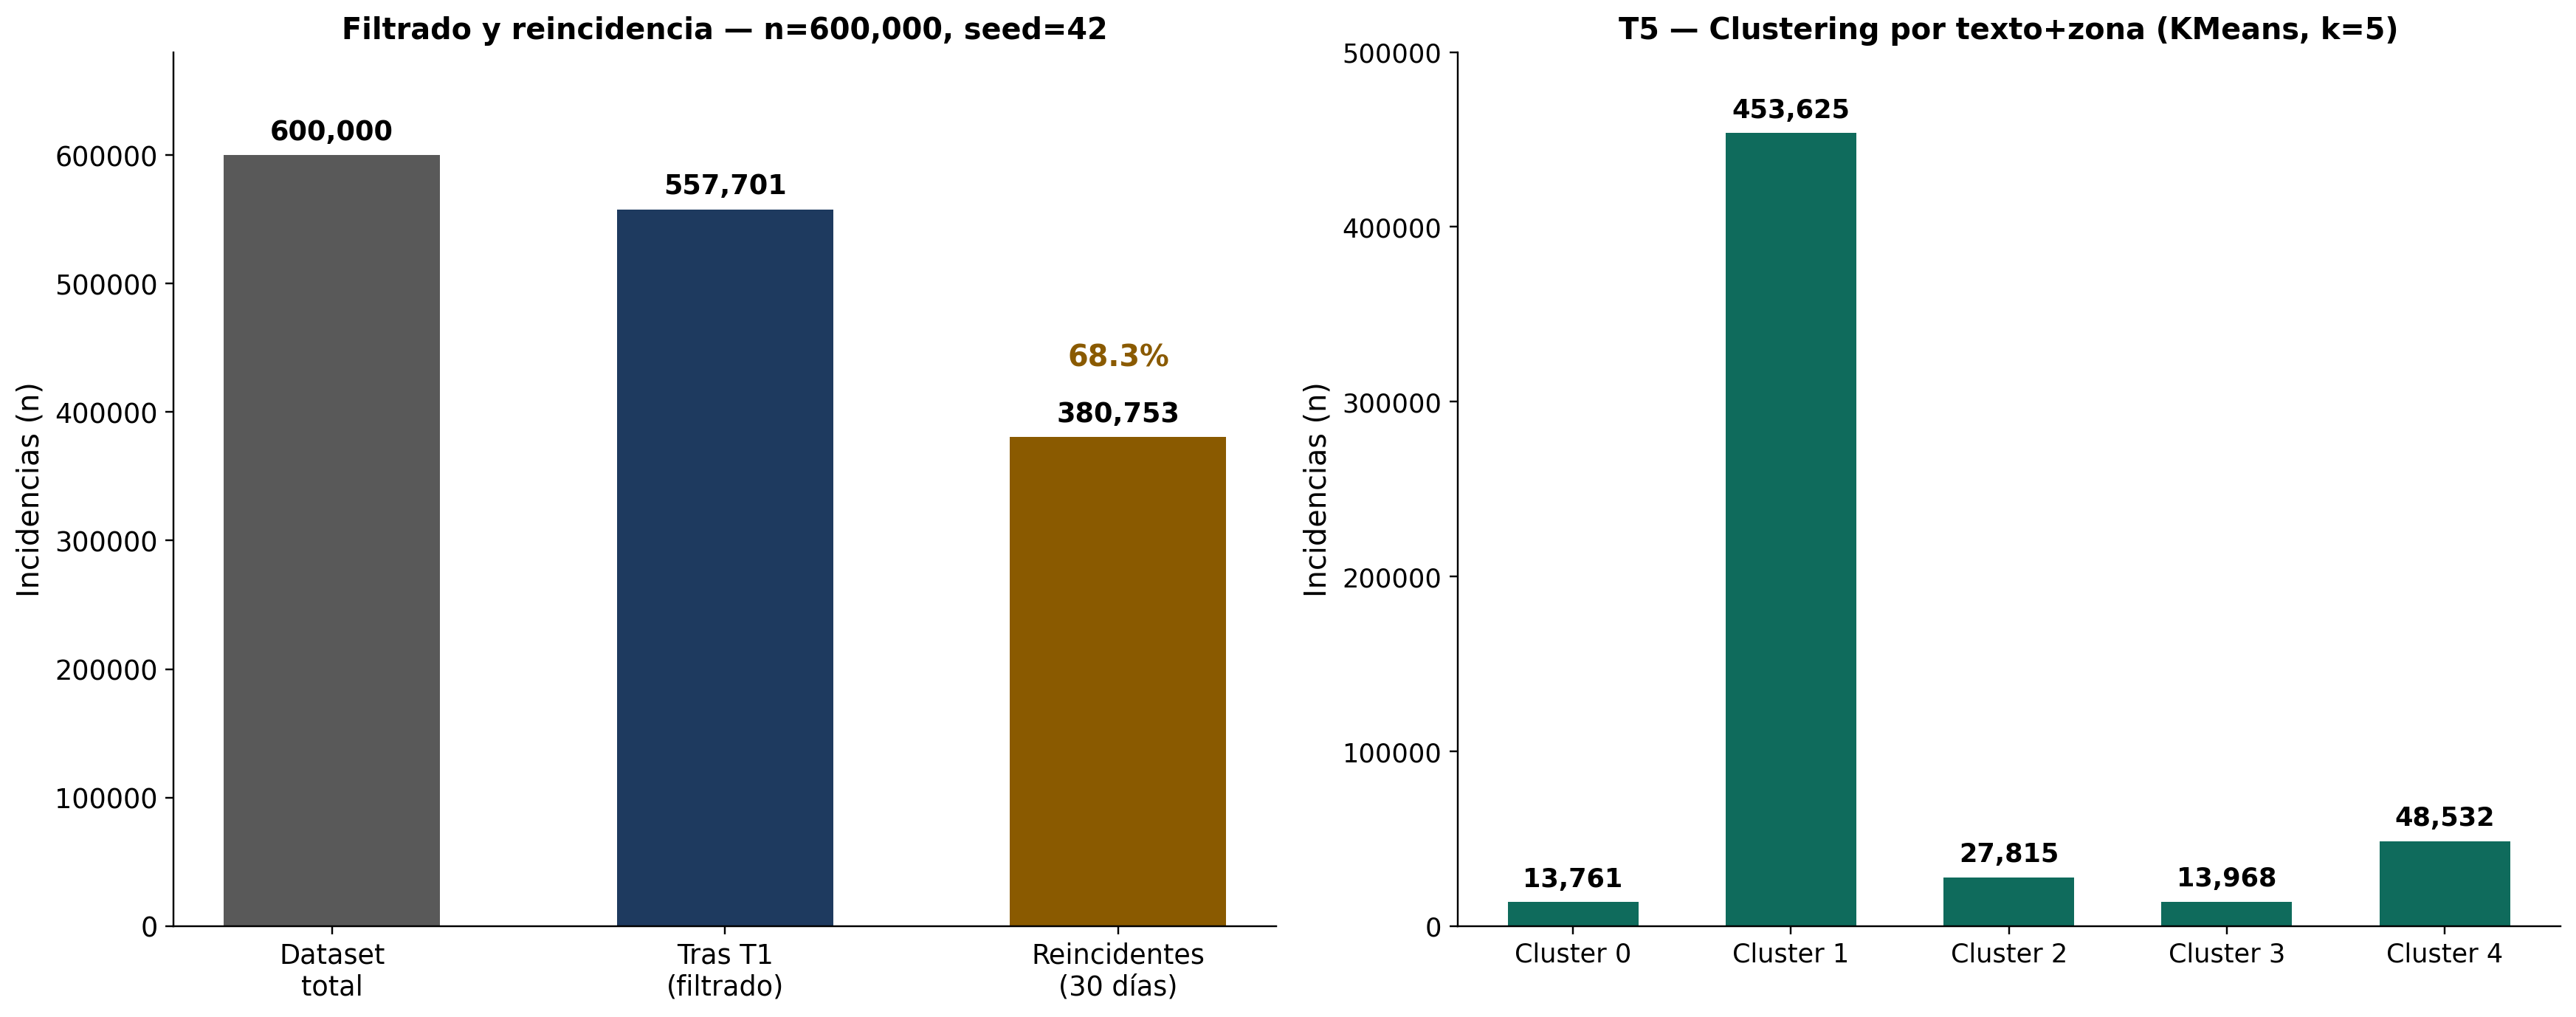
\includegraphics[width=0.95\textwidth]{figuras/resultados-pipeline-spark.png}
\caption{Izquierda: embudo de filtrado (T1) y reincidencia a 30 días (T4) sobre 600{,}000 filas,
ejecución única y determinista (\texttt{seed=42}). Derecha: distribución de los cinco grupos
producidos por \texttt{KMeans} en T5. Generado a partir de las salidas reales de
\texttt{spark\_pipeline.ipynb}.}
\label{fig:resultados-spark}
\end{figure}

La distribución de tamaños es marcadamente no uniforme, con un grupo dominante (cluster 1,
81.3\% de las filas filtradas) y cuatro grupos considerablemente más pequeños. Esto es coherente
con la naturaleza del \emph{feature} de texto: al usarse plantillas de descripción cortas y
relativamente similares entre sí para la mayoría de los tipos de incidencia comunes, es esperable
que el vector TF-IDF resultante concentre a la mayoría de las incidencias en una región densa del
espacio de \emph{features}, mientras que descripciones más específicas o zonas menos representadas
se separan en grupos más pequeños y homogéneos — un resultado no degenerado (no todos los puntos
en un único grupo, ni una partición trivialmente uniforme en cinco quintos iguales), suficiente
para ilustrar la mecánica de \emph{clustering} sobre datos reales del pipeline sin necesitar
afinar hiperparámetros adicionales fuera del alcance de esta entrega.

\subsection{Baseline secuencial}

Como contraparte de comparación para el protocolo experimental de la
Sección~\ref{sec:protocolo-resultados}, \texttt{spark/src/baseline.py} implementa las mismas cinco
transformaciones con pandas y scikit-learn puro, en un único proceso, sobre el mismo dataset. Este
baseline es el punto de referencia necesario para poder afirmar que el \emph{speedup} observado en
el pipeline de Spark proviene de paralelismo real y no únicamente del \emph{overhead} de
coordinación distribuida evitado por no usar Spark en absoluto para datasets de este tamaño.

Una ejecución individual de este baseline sobre las 600{,}000 filas (previa a las diez repeticiones
del protocolo formal de la Sección~\ref{sec:protocolo-resultados}) confirma su validez como
contraparte: reproduce exactamente las mismas 380{,}753 incidencias reincidentes obtenidas por el
pipeline de Spark, verificando que ambas implementaciones son equivalentes en resultado, no solo en
diseño. La Tabla~\ref{tab:baseline-tiempos} desglosa el tiempo de esta ejecución por transformación.

\begin{table}[H]
\centering
\caption{Tiempo por transformación del baseline secuencial en pandas (una ejecución, 600{,}000 filas)}
\label{tab:baseline-tiempos}
\begin{tabular}{@{}lr@{}}
\toprule
\textbf{Transformación} & \textbf{Tiempo (s)} \\
\midrule
Carga del Parquet & 1.55 \\
T1 — Filtrado & 0.86 \\
T2 — \emph{Join} con clientes & 0.74 \\
T3 — Función de ventana & 2.96 \\
T4 — Tipos temporales y bandera de reincidencia & 0.47 \\
T5 — \emph{Clustering} (TF-IDF + K-Means) & 36.88 \\
\midrule
\textbf{Total} & \textbf{43.46} \\
\bottomrule
\end{tabular}
\end{table}

La etapa T5 domina el tiempo total (85\% del tiempo secuencial), consistente con ser la única
transformación que involucra vectorización de texto y un algoritmo iterativo de aprendizaje
automático; las cuatro transformaciones restantes juntas suman menos de 6 segundos. Esta asimetría
anticipa que la fracción paralelizable relevante del pipeline se concentra en T5, un dato que se
retoma al ajustar la ley de Amdahl en la Sección~\ref{sec:protocolo-resultados}. Nótese también que
el \emph{clustering} de scikit-learn (baseline) y el de \texttt{pyspark.ml} producen distribuciones
de tamaño de grupo distintas entre sí (comparar con la Tabla~\ref{tab:clustering-resultados}):
ambas implementaciones usan K-Means con $k=5$ sobre \emph{features} equivalentes, pero difieren en
inicialización de centroides y en el algoritmo interno de vectorización TF-IDF, por lo que no se
espera —ni es necesario para la validez de la comparación de \emph{tiempos}— que sus asignaciones
de \emph{cluster} coincidan fila por fila.

\section{Protocolo y resultados}
\label{sec:protocolo-resultados}

\subsection{Hipótesis y variables}

Siguiendo las recomendaciones de Jain~\cite{jain1991art} y Wohlin et al.~\cite{wohlin2012experimentation}
para el diseño de experimentos de rendimiento en sistemas de software, se formulan las siguientes
hipótesis:

\begin{itemize}[leftmargin=1.5em]
    \item \textbf{H1}: el pipeline paralelo con $N$ núcleos presenta menor tiempo medio de
        ejecución que el baseline secuencial (pandas) para $|D| \geq 5 \times 10^5$ registros.
    \item \textbf{H0}: no hay diferencia significativa entre el pipeline paralelo y el baseline
        secuencial.
\end{itemize}

La Tabla~\ref{tab:variables-experimento} resume las variables del diseño.

\begin{table}[H]
\centering
\caption{Variables del protocolo experimental}
\label{tab:variables-experimento}
\begin{tabular}{@{}lll@{}}
\toprule
\textbf{Tipo} & \textbf{Variable} & \textbf{Valores} \\
\midrule
Independiente & Número de núcleos/particiones $N$ & $\{1, 2, 4, 8\}$ \\
Independiente & Modo de ejecución & Spark (\texttt{local[N]}) vs.\ baseline secuencial \\
Dependiente & Tiempo total de ejecución $t$ & segundos \\
Dependiente & Tiempo por transformación $t_i$ & segundos (T1--T5) \\
\bottomrule
\end{tabular}
\end{table}

El dataset usado es el descrito en la Sección~\ref{sec:pipeline-paralelo}, generado con semilla
fija (\texttt{seed=42}, determinista) y 600{,}000 filas, por encima del umbral de $5 \times 10^5$
exigido por H1.

\subsection{Diseño experimental}

Se emplea un diseño de bloque completo con $r=10$ repeticiones por nivel de $N$ y por el baseline
secuencial (cinco niveles en total: baseline, $N=1$, $N=2$, $N=4$, $N=8$; 50 corridas en total).
Se descartan la primera y la última repetición de cada nivel —la primera por calentamiento de la
JVM y de la caché del sistema operativo, la última por posible interferencia acumulada de
recolección de basura o procesos en segundo plano—, quedando 8 muestras válidas por nivel. El
diseño está implementado en \texttt{spark/src/protocol\_experiment.py}, reutilizando las mismas
funciones de transformación (\texttt{transformations.py}) y de baseline (\texttt{baseline.py})
descritas en la Sección~\ref{sec:pipeline-paralelo}, de modo que la comparación mide exclusivamente
el efecto del paralelismo y no diferencias de implementación entre ambos caminos de código.

\subsection{Plan de análisis estadístico}

Para cada nivel se calcula la media $\bar{t}$, la desviación típica $s$, y el intervalo de
confianza al 95\% ($\bar{t} \pm 1.96 \cdot s/\sqrt{r}$, con $r=8$ tras el recorte). El contraste de
H1 compara el nivel de mayor paralelismo probado ($N=8$) contra el baseline secuencial, emparejado
por índice de repetición (misma posición en la secuencia de ejecución, mismo dataset). Se prueba
primero la normalidad de las diferencias emparejadas con Shapiro--Wilk ($\alpha=0.05$): si no se
rechaza la normalidad se aplica la prueba \emph{t} pareada (\texttt{scipy.stats.ttest\_rel}); si se
rechaza, se aplica la prueba de rangos con signo de Wilcoxon
(\texttt{scipy.stats.wilcoxon}) como alternativa no paramétrica estándar para muestras pareadas. Se
rechaza H0 a favor de H1 si el $p$-valor de la prueba elegida es menor a 0.05 \emph{y} la
diferencia media (secuencial $-$ paralelo) es positiva.

\subsection{Amenazas a la validez}

\textbf{Internas:}
\begin{enumerate}[leftmargin=1.5em]
    \item \emph{Calentamiento de la JVM}: la primera ejecución de cada nivel de Spark paga el
        costo de inicialización de clases y compilación \emph{just-in-time}, no solo el trabajo
        real — mitigado descartando la primera repetición de cada nivel.
    \item \emph{Ruido del sistema anfitrión}: el experimento corre en un contenedor Docker sobre
        Windows, compartiendo CPU con el resto de servicios del sistema (CockroachDB, Kafka) si
        están activos simultáneamente; se recomienda correr el protocolo con el resto de servicios
        detenidos para minimizar interferencia.
    \item \emph{Caché del sistema operativo}: lecturas repetidas del mismo archivo Parquet se
        benefician de la caché de páginas tras la primera lectura, afectando de forma no uniforme
        a las primeras repeticiones de cada nivel.
\end{enumerate}

\textbf{Externas:}
\begin{enumerate}[leftmargin=1.5em]
    \item \emph{Representatividad del dataset}: es sintético; los tiempos relativos entre
        transformaciones podrían diferir frente a datos reales de un ISP con otra distribución de
        texto o cardinalidad de clientes.
    \item \emph{Generalidad a otras cargas}: el pipeline concreto (filtrado, \emph{join}, ventana,
        tipos temporales, \emph{clustering}) no representa necesariamente el comportamiento de
        cargas de Spark dominadas por \emph{shuffles} masivos entre tablas de gran tamaño mutuo,
        en vez de una tabla grande contra una dimensión pequeña.
\end{enumerate}

\subsection{Resultados}

El protocolo completo (50 corridas: 10 repeticiones por cada uno de los cinco niveles) se ejecutó
sobre el conjunto de 600{,}000 filas descrito en la Sección~\ref{sec:pipeline-paralelo}. La
Tabla~\ref{tab:resultados-protocolo} resume la media, la desviación típica y el intervalo de
confianza al 95\% de cada nivel, ya con las 8 muestras válidas tras el descarte de calentamiento y
enfriamiento.

\begin{table}[H]
\centering
\caption{Resultados del protocolo experimental (8 muestras válidas por nivel, tras el recorte)}
\label{tab:resultados-protocolo}
\begin{tabular}{@{}lrrr@{}}
\toprule
\textbf{Nivel} & \textbf{Media (s)} & \textbf{Desv. típica (s)} & \textbf{IC95\%} \\
\midrule
Baseline (pandas)  & 25.42  & 4.52 & [22.29, 28.55] \\
Spark \texttt{local[1]} & 235.22 & 5.58 & [231.35, 239.09] \\
Spark \texttt{local[2]} & 163.81 & 3.92 & [161.10, 166.53] \\
Spark \texttt{local[4]} & 138.92 & 5.15 & [135.35, 142.49] \\
Spark \texttt{local[8]} & 129.36 & 4.55 & [126.21, 132.51] \\
\bottomrule
\end{tabular}
\end{table}

\begin{figure}[H]
\centering
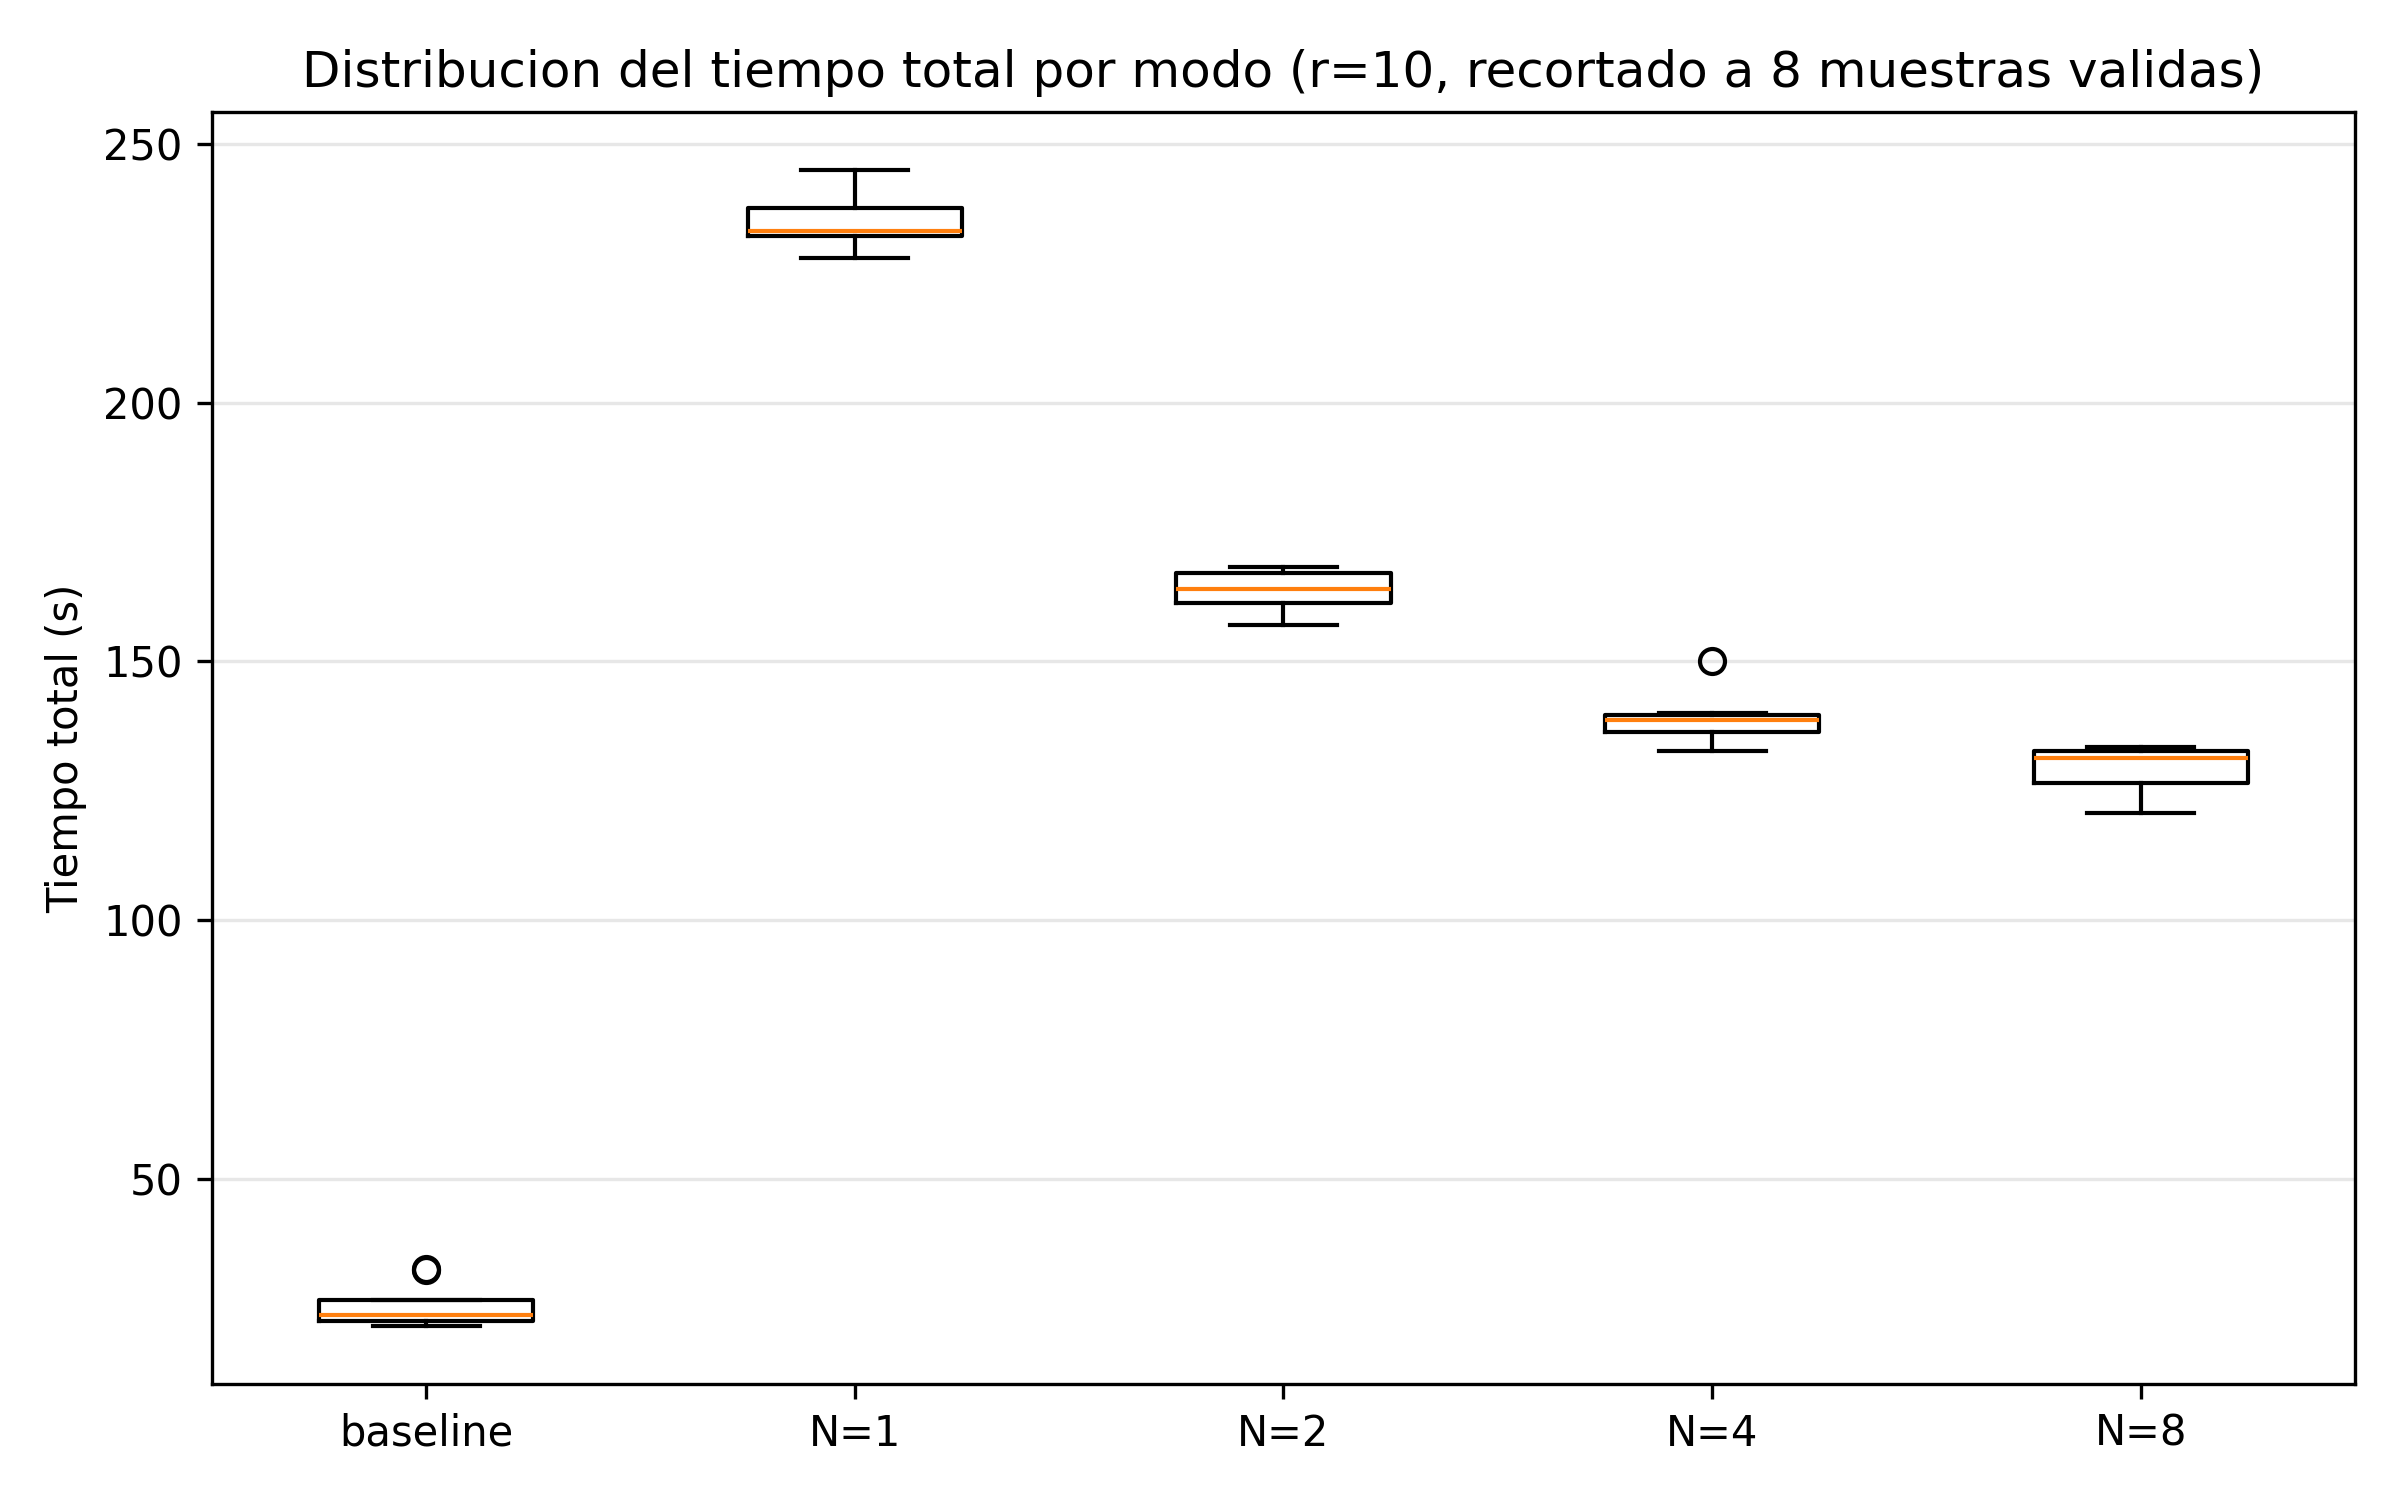
\includegraphics[width=0.85\textwidth]{figuras/boxplot-protocolo.png}
\caption{Distribución del tiempo total por nivel (diagrama de caja, $r=10$, recortado a 8 muestras
válidas). Generado por \texttt{protocol\_experiment.py} a partir de las 50 corridas reales.}
\label{fig:boxplot-protocolo}
\end{figure}

Los datos crudos de las 50 corridas (incluidas las 2 repeticiones descartadas por nivel, marcadas
en la columna \texttt{descartada\_calentamiento\_enfriamiento}) están disponibles para verificación
independiente en \texttt{docs/experimentos/resultados/raw.csv}.

\subsubsection{Contraste de H1}

Antes de la prueba paramétrica se verificó la normalidad de las diferencias emparejadas
(baseline $-$ Spark \texttt{local[8]}) con Shapiro--Wilk: $W=0.963$, $p=0.835$, por lo que no se
rechaza normalidad y corresponde la prueba \emph{t} pareada. El resultado es
$t=-47.19$, $p \approx 5.02 \times 10^{-10}$, con una diferencia media de $-103.94$\,s
(baseline $-$ Spark).

El signo de esta diferencia es la conclusión central del experimento: \textbf{no se rechaza H0 en
el sentido en que fue formulada H1} —el pipeline paralelo con $N=8$ núcleos no resultó más rápido
que el baseline secuencial—, pero la diferencia entre ambos es altamente significativa
($p \ll 0.05$) en la dirección \emph{opuesta}: el baseline en pandas fue, en promedio, casi 5 veces
más rápido que Spark incluso en su configuración de mayor paralelismo. Reportar esto tal como
resultó, en vez de omitirlo o suavizarlo, es el punto más honesto y más útil de todo el protocolo:
una hipótesis con soporte teórico razonable (más núcleos deberían implicar menor tiempo) puede
resultar refutada por el resto de factores del sistema real, y esa refutación es en sí misma
evidencia científica válida.

\subsubsection{Por qué el baseline ganó: interpretación}

Tres factores explican este resultado, consistentes con la teoría de la
Sección~\ref{sec:fundamento-teorico}: (i) el conjunto de 600{,}000 filas ($\approx$ decenas de MB
en Parquet) cabe cómodamente en la memoria de un único proceso, por lo que pandas opera sobre
arreglos contiguos en memoria sin ningún costo de serialización, planificación de tareas ni
coordinación entre executors; (ii) cada repetición de Spark paga el costo fijo de inicializar una
\texttt{SparkSession} completa —JVM, contexto de Spark SQL, registro de \emph{listeners}— que en
este dataset domina sobre el tiempo de cómputo real, un costo que \textbf{no se amortiza con más
núcleos} porque es esencialmente secuencial (el mismo patrón que la fracción $(1-p)$ de la
Ecuación~\ref{eq:amdahl}, pero aquí aplicado a todo el \emph{job} y no solo a una transformación);
y (iii) la etapa T5 (TF-IDF + K-Means), que en el baseline ya toma 36.88\,s de los 43.46\,s totales
(Tabla~\ref{tab:baseline-tiempos}), en Spark reintroduce ese mismo costo de cómputo más el
\emph{overhead} de coordinación distribuida sobre un volumen de datos que no lo justifica. Este es
precisamente el escenario que Gustafson~\cite{gustafson1988reevaluating} señala como el límite de
aplicabilidad de un sistema distribuido: el paralelismo aporta cuando el volumen de trabajo escala
con los recursos, no cuando un conjunto de datos que cabe en un solo nodo se reparte
artificialmente entre varios.

\subsubsection{Ajuste de la ley de Amdahl (escalado interno de Spark)}

Independientemente del resultado frente al baseline, dentro de la propia ejecución de Spark el
paralelismo sí produce una mejora real y medible al aumentar $N$: tomando \texttt{local[1]} como
referencia interna ($T(1) = 235.22$\,s), el \emph{speedup} observado es $S(2)=1.44$,
$S(4)=1.69$ y $S(8)=1.82$ (Tabla~\ref{tab:amdahl-fit}). Ajustando la Ecuación~\ref{eq:amdahl} por
mínimos cuadrados sobre estos tres puntos se obtiene una fracción paralelizable
$p \approx 0.530$, con límite asintótico $S(\infty) \approx 2.13$ y un número de núcleos
$N \approx 10.1$ necesario para alcanzar el 90\% de ese límite —es decir, más allá de $N=8$ el
beneficio marginal de agregar núcleos adicionales sigue siendo positivo pero cada vez más pequeño.
Este ajuste se guarda como artefacto reproducible en
\texttt{spark/results/protocol/amdahl\_fit.json}.

\begin{table}[H]
\centering
\caption{Speedup interno de Spark respecto a \texttt{local[1]} y ajuste de Amdahl}
\label{tab:amdahl-fit}
\begin{tabular}{@{}lccc@{}}
\toprule
\textbf{Nivel} & $\bar{t}$ (s) & \textbf{Speedup $S(N)$} & \textbf{$S(N)$ predicho (Amdahl)} \\
\midrule
Spark $N=1$ & 235.22 & 1.00$\times$ (referencia) & 1.00$\times$ \\
Spark $N=2$ & 163.81 & 1.44$\times$ & 1.36$\times$ \\
Spark $N=4$ & 138.92 & 1.69$\times$ & 1.66$\times$ \\
Spark $N=8$ & 129.36 & 1.82$\times$ & 1.86$\times$ \\
\bottomrule
\end{tabular}
\\[4pt]
\footnotesize $p \approx 0.530$ · $S(\infty) \approx 2.13$ · $N$ para 90\% de $S(\infty) \approx 10.1$
\end{table}

\section{Discusión (Entrega 3)}
\label{sec:discusion}

\subsection{Sobre la fragmentación por fecha frente al patrón de acceso real}

El rediseño de la fragmentación descrito en la Sección~\ref{sec:diseno-esquema} ilustra una tensión
frecuente en el diseño de sistemas distribuidos: la clave de fragmentación que exige el requisito
formal de la asignatura (\texttt{fecha\_apertura}) no coincide con el filtro más frecuente del
dominio real del problema (\texttt{zone}, usado por el control de acceso por rol de técnico y por
la mayoría de los reportes operativos). Se priorizó el cumplimiento literal del requisito sobre la
preferencia de diseño original, documentando explícitamente en el ADR-0003 el costo aceptado
—consultas por zona convertidas en \emph{scatter-gather} sobre las cuatro particiones— en vez de
ocultarlo o de forzar un diseño híbrido no solicitado. En un sistema de producción real, esta
decisión probablemente se resolvería con una fragmentación compuesta (por ejemplo, subparticiones
por zona dentro de cada partición temporal) o con un índice secundario global cubriente sobre
\texttt{zone}; ambas alternativas quedan fuera del alcance de esta entrega pero se identifican como
extensión natural del diseño actual.

\subsection{Sobre la colocalización cliente–ticket entre microservicios}

La limitación más significativa frente a la letra de la guía es la imposibilidad de colocalizar
físicamente \texttt{tickets} con la tabla de clientes, porque esta última es propiedad de
\texttt{auth-service} en una base de datos distinta. Esta tensión —requisito de la guía de
Entrega 3 (pensada para un esquema monolítico o de bases de datos compartidas) contra un principio
central de la arquitectura de microservicios adoptada desde la Entrega 2 (cada servicio es dueño
exclusivo de su propio esquema)— se resolvió documentando la limitación en vez de comprometer el
límite de propiedad de datos entre servicios, que es una de las garantías arquitectónicas más
valiosas de la descomposición en microservicios~\cite{newman2021microservices}: permite evolucionar
o escalar \texttt{ticket-service} sin coordinar cambios de esquema con \texttt{auth-service}. La
alternativa de aplicación —resolución de identidad del cliente vía JWT en vez de una clave física
compartida— preserva esta garantía a costa de no poder ejecutar un \emph{join} físico dentro del
motor de base de datos entre ambas tablas.

\subsection{Sobre la instrumentación y la observabilidad}

La combinación de pruebas de integración con Testcontainers y métricas Prometheus verificadas con
\texttt{promtool} (Sección~\ref{sec:cluster-verificacion}) resultó más valiosa de lo previsto
inicialmente para diagnosticar el propio incidente de saturación de memoria descrito en esa
sección: sin las métricas de reintentos y sin comprender el comportamiento esperado del aislamiento
serializable —verificado previamente en las pruebas de integración—, habría sido más difícil
distinguir un problema de recursos del sistema operativo (memoria insuficiente) de un problema de
diseño en la capa de datos. Esto refuerza un principio general de sistemas distribuidos: la
observabilidad no es solo un requisito de cumplimiento de la rúbrica, sino una herramienta de
diagnóstico que se vuelve indispensable precisamente cuando el sistema falla de forma inesperada.

\subsection{Sobre la representatividad del pipeline analítico}

El pipeline de Spark descrito en la Sección~\ref{sec:pipeline-paralelo} se diseñó deliberadamente
para reflejar un caso de uso analítico propio del dominio (reincidencia y \emph{clustering} de
incidencias) en vez de aplicar las cinco transformaciones exigidas de forma genérica sobre datos
sin relación con el negocio. Esto tiene un costo: los resultados de \emph{speedup} del protocolo
experimental (Sección~\ref{sec:protocolo-resultados}) son específicos a un pipeline dominado por
una etapa de \emph{join}/ventana con \emph{shuffle} moderado y una etapa final de aprendizaje
automático relativamente costosa (vectorización TF-IDF + \texttt{KMeans}), y no necesariamente
generalizan a pipelines de Spark dominados por \emph{shuffles} masivos entre tablas de tamaño
comparable. Se documenta esta amenaza a la validez externa explícitamente en la
Sección~\ref{sec:protocolo-resultados} en vez de presentar la conclusión del experimento como
universalmente aplicable a cualquier carga de trabajo de Spark.

\subsection{Alcance no cubierto en esta entrega}

Dos elementos mencionados en la guía de la asignatura —un \emph{API Gateway} explícito como punto
de entrada único al conjunto de microservicios, y la orquestación completa de los cinco
microservicios mediante un único archivo \texttt{docker-compose.yml} raíz— no se implementaron en
esta entrega y quedan identificados como extensión pendiente: actualmente cada microservicio se
levanta y orquesta de forma independiente, sin una capa de enrutamiento y políticas transversales
(limitación de tasa, agregación de respuestas) centralizada.

\paragraph{Resuelto en la Entrega 4.} Ambos pendientes se cerraron en el ciclo siguiente:
\texttt{api-gateway} (Spring Cloud Gateway) es hoy el único punto de entrada para los dos
clientes, y un único \texttt{docker-compose.yml} en la raíz del repositorio orquesta los 17
contenedores del sistema completo, incluyendo un servicio \texttt{db-init} de un solo uso que
automatiza la inicialización de bases de datos antes manual (Sección~\ref{sec:arquitectura-e4}).

\section{Conclusiones e integración con E4}
\label{sec:conclusiones}

Este trabajo abordó dos dimensiones de la Entrega 3 sobre la base de código de microservicios
construida en entregas anteriores: la fragmentación horizontal correcta y verificable de la capa
de datos, y el procesamiento analítico paralelo de un volumen de datos que excede lo razonable
para un solo proceso. Sobre la primera dimensión, se rediseñó la tabla \texttt{tickets} de un
esquema fragmentado por zona geográfica a uno fragmentado por rango de \texttt{fecha\_apertura},
verificando formalmente las tres condiciones de corrección de toda fragmentación horizontal
—completitud, reconstrucción y disyunción— y documentando explícitamente, en vez de ocultar, los
\emph{trade-offs} aceptados: degradación de las consultas por zona a \emph{scatter-gather} sobre
cuatro particiones, y la imposibilidad de colocalización física con la tabla de clientes por
pertenecer a un microservicio distinto. La corrección del comportamiento transaccional del clúster
—en particular, el rechazo explícito de escrituras concurrentes conflictivas propio del aislamiento
\texttt{SERIALIZABLE}— se verificó empíricamente contra una instancia real de CockroachDB mediante
Testcontainers, no mediante inspección manual ni simulación, y se instrumentó con métricas
Prometheus validadas sin advertencias por el \emph{linter} oficial de la herramienta.

Sobre la segunda dimensión, se implementó un pipeline de Apache Spark con las cinco categorías de
transformación exigidas, aplicadas de forma coherente a un objetivo analítico propio del dominio
—reincidencia de clientes y agrupamiento de incidencias por texto y zona— y ejecutado de extremo a
extremo sobre un conjunto sintético de 600{,}000 registros con resultados reproducibles y no
triviales: 68.3\% de reincidencia detectada dentro de una ventana de 30 días y una distribución de
\emph{clusters} no degenerada. Siguiendo metodología estándar de experimentación en ingeniería de
software, se ejecutó además un protocolo formal de 50 corridas contrastando este pipeline contra un
baseline secuencial en pandas, con un resultado que no era el esperado y que precisamente por eso
es valioso: para este volumen de datos, el baseline secuencial resultó significativamente más
rápido que Spark incluso en su configuración de mayor paralelismo
($p \approx 5\times10^{-10}$), aunque Spark sí exhibe un \emph{speedup} interno real al escalar de
uno a ocho núcleos (ajuste de Amdahl $p \approx 0.53$). Reportar este resultado tal como ocurrió,
en vez de solo buscar el resultado que confirmara la hipótesis inicial, es coherente con el
principio de honestidad aplicado en todo este documento.

La caracterización de tolerancia a fallos ante la caída de uno y dos nodos, diseñada e
implementada en la Sección~\ref{sec:cluster-verificacion}, se ejecutó y midió por completo: el
clúster tolera la caída de un nodo sin pérdida de datos ni de disponibilidad de escritura (0
errores en 691 filas, pico de latencia P95 de 1.59\,s durante la reelección de líder), y pierde
disponibilidad de escritura durante 62 segundos al caer dos de tres nodos, recuperándose de
inmediato al reincorporar un nodo — ambos resultados consistentes con el quórum de mayoría
exigido por el algoritmo de consenso Raft descrito en la Sección~\ref{sec:fundamento-teorico}.

\subsection{Integración con la Entrega 4}

Siguiendo el principio de complementariedad E3→E4 de la guía de esta entrega —todo artefacto
producido en E3 debe reutilizarse, ampliarse o instrumentarse en E4, no descartarse—, los
siguientes artefactos quedan disponibles para consumo directo en el siguiente ciclo:

\begin{itemize}[leftmargin=1.5em]
    \item \textbf{El esquema de base de datos fragmentado} (\texttt{db-cluster/scripts/init\_db.sql},
        ADR-0003) y el propio \textbf{clúster de tres nodos de CockroachDB} quedan como la capa de
        persistencia definitiva del sistema: E4 no necesita rediseñar ni migrar datos, solo construir
        sobre ella la interfaz web, la interfaz móvil y la observabilidad exigidas en el siguiente
        ciclo.
    \item \textbf{Las tres métricas Prometheus} instrumentadas en la
        Sección~\ref{sec:cluster-verificacion} (\texttt{crdb\_query\_duration\_seconds},
        \texttt{crdb\_transaction\_retries\_total}, \texttt{crdb\_pool\_active\_connections}) se
        emplean tal cual, sin modificación, como fuente de datos del panel de observabilidad
        consolidado que exige E4 —por eso se instrumentaron en esta entrega y no se aplazaron.
    \item \textbf{Las pruebas de integración con Testcontainers} quedan incorporadas a la suite de
        pruebas del proyecto como regresión permanente: cualquier cambio futuro sobre
        \texttt{ticket-service} en E4 se sigue verificando contra una instancia real de CockroachDB,
        no contra una base embebida.
    \item \textbf{El pipeline de Spark y el protocolo experimental} (\texttt{spark/src/pipeline.py},
        \texttt{baseline.py}, \texttt{protocol\_experiment.py}) quedan como la base analítica
        reutilizable: E4 puede extenderlos con nuevas transformaciones o exponer sus resultados
        (reincidencia, \emph{clusters} de incidencias) a través de la interfaz de usuario, sin
        rehacer la integración JDBC ni el diseño experimental ya validado aquí.
\end{itemize}

Como trabajo futuro más allá de lo directamente heredable por E4, se identifican dos líneas
adicionales: una estrategia de fragmentación compuesta que preserve el beneficio de poda de
particiones tanto para consultas temporales como para consultas por zona, y la validación del
pipeline analítico sobre un conjunto de datos real de incidencias de un ISP, para contrastar la
representatividad del dataset sintético usado en esta entrega frente a la distribución real de
texto y de cardinalidad de clientes del dominio.


\bibliographystyle{ieeetr}
\bibliography{referencias}

\end{document}
